% ============================================================
% SECTION 4 - KIẾN TRÚC KỸ THUẬT
% Nền tảng · Kiến trúc ba lớp · Mô-đun · Điều hướng
% Dữ liệu · Upload & phát · Lưu trữ · Phối hợp media · TTS
% ============================================================
\section{Kiến trúc kỹ thuật}

% ------------------------------------------------------------
\subsection{Nền tảng và lựa chọn kỹ thuật}
% ------------------------------------------------------------
\begin{frame}{Nền tảng và lựa chọn kỹ thuật}
\small
\centering
\begin{tabular}{@{}p{3.4cm}p{5.3cm}p{5.2cm}@{}}
\toprule
\textbf{Vai trò} & \textbf{Công nghệ} & \textbf{Mục đích} \\
\midrule
Nền tảng và giao diện & Android, Kotlin, Compose, Material 3 & Xây dựng giao diện và tích hợp Android \\
Trạng thái và lắp ghép & ViewModel, StateFlow, Hilt & Quản lý UI state và cung cấp thành phần \\
Điều hướng và phát media & Navigation Compose, Media3 & Chuyển màn hình, dùng chung bộ phát \\
Kết nối và lưu dữ liệu & Retrofit, Room, DataStore & Gọi API, lưu dữ liệu và thiết lập \\
\bottomrule
\end{tabular}

\vspace{0.3cm}
\begin{exampleblock}{Lý do chọn Android Native}
Kotlin + Jetpack Compose: một hệ công cụ duy nhất cho cả bốn phân hệ; một vòng đời, một audio focus; Media3 là bộ phát dùng chung; nhóm đã có kinh nghiệm. Hỗ trợ tối thiểu \textbf{Android 8.0 (API 26)}.
\end{exampleblock}
\end{frame}

% ------------------------------------------------------------
\subsection{Lý giải lựa chọn công nghệ}
% ------------------------------------------------------------
\begin{frame}{Lý giải lựa chọn công nghệ --- các phương án đã cân nhắc}
\begin{center}\tiny
\setlength{\tabcolsep}{3pt}
\begin{tabular}{@{}p{2.4cm}p{4.6cm}p{4.0cm}p{2.4cm}@{}}
\toprule
\textbf{Phương án} & \textbf{Điểm phù hợp} & \textbf{Chi phí trong bài} & \textbf{Kết luận} \\
\midrule
\textbf{Android Native / Kotlin} & Trực tiếp dùng lifecycle, Media3, media session và audio focus; nhóm có kinh nghiệm & Chỉ triển khai Android & \textbf{Chọn} \\
iOS Native / Swift & Tích hợp hệ thống iOS trực tiếp & Thêm nền tảng và công cụ; không có bản iOS để kiểm thử & Phân tích, không triển khai \\
Flutter & Chia sẻ UI và logic đa nền tảng & Cần kiểm tra plugin và phần tích hợp Android cho từng yêu cầu media & Không chọn trong phạm vi bài \\
React Native & Chia sẻ UI/logic bằng JS/TS & Phụ thuộc thư viện / native integration cho media và background & Không chọn \\
Kotlin Multiplatform & Chia sẻ logic Kotlin & Vẫn cần chiến lược UI/media theo nền tảng; tăng phạm vi kiểm thử & Cân nhắc sau nếu có iOS \\
\bottomrule
\end{tabular}
\end{center}
\vspace{1.2mm}
{\tiny\color{TextGray} Lý do cốt lõi: bài tập trung vào \textbf{vòng đời, đa nhiệm media và audio focus}~--~những thứ cần quyền truy cập hệ thống sâu nhất. Không khẳng định framework này luôn nhanh hơn framework khác, hay mọi app đa nền tảng đều phải tự viết native bridge.}
\end{frame}

% ------------------------------------------------------------
\subsection{Kiến trúc tổng thể}
% ------------------------------------------------------------
\begin{frame}{Kiến trúc tổng thể: app, backend và dịch vụ ngoài}
\begin{center}
\begin{tikzpicture}[
  font=\scriptsize,
  box/.style={draw=BKTemplate, thick, rounded corners=3pt, fill=BKTemplate!8, align=center, inner sep=3pt},
  ext/.style={draw=GreenOK!70!black, thick, rounded corners=3pt, fill=GreenOK!8, align=center, inner sep=3pt},
  lnk/.style={-{Latex[length=1.8mm]}, thick, BKTemplate!80},
  lnk2/.style={-{Latex[length=1.8mm]}, thick, dashed, TextGray}]
  \node[box, minimum width=4.0cm, minimum height=0.85cm] (tts) at (2.55,6.3) {\textbf{TTS on-device / cloud}\\{\tiny module thay được}};
  \node[box, minimum width=4.6cm, minimum height=3.4cm] (app) at (2.55,3.15) {\textbf{Ứng dụng Android}\\[2pt]
    Compose UI $\cdot$ ViewModel\\
    Media3 player (dùng chung)\\
    Room $\cdot$ DataStore\\[2pt]
    {\tiny feature: video $\cdot$ nhạc $\cdot$ tin $\cdot$ game $\cdot$ dùng chung}};
  \node[box, minimum width=3.8cm, minimum height=1.1cm] (api) at (9.55,4.75) {\textbf{API server (thiết kế)}\\REST $\cdot$ JSON};
  \node[box, minimum width=3.8cm, minimum height=1.1cm] (db) at (9.55,2.3) {\textbf{CSDL quan hệ + kho media}\\dữ liệu $\cdot$ tệp phát};
  \node[ext, minimum width=2.0cm, minimum height=1.1cm] (rss) at (12.75,4.75) {\textbf{RSS}\\VnExpress};
  \draw[lnk] ([yshift=14pt]app.east) -- ([yshift=6pt]api.west) node[midway, above, font=\tiny, align=center]{HTTPS/JSON: danh mục\\$\cdot$ tài khoản $\cdot$ điểm};
  \draw[lnk] ([yshift=-14pt]app.east) -- ([yshift=-4pt]db.west) node[midway, below, font=\tiny]{HTTPS stream media (Media3)};
  \draw[lnk] (api.south) -- (db.north) node[midway, right, font=\tiny]{SQL};
  \draw[lnk2] (rss.west) -- (api.east) node[midway, above, font=\tiny]{nạp tin};
  \draw[lnk, {Latex[length=1.8mm]}-{Latex[length=1.8mm]}] (app.north) -- (tts.south) node[midway, right, font=\tiny]{đọc bài};
\end{tikzpicture}
\end{center}
\vspace{1mm}
{\tiny\color{TextGray} Sơ đồ mức \textbf{container (C4)}. Giai đoạn môn học: \textbf{local-first}~--~danh mục do repository trong app cung cấp (mock), backend hoãn theo ADR-17. Thay nguồn $=$ thay URL: player, UI và logic phát không đổi.}
\end{frame}

% ------------------------------------------------------------
\subsection{Kiến trúc ba lớp}
% ------------------------------------------------------------
\begin{frame}{Kiến trúc ba lớp}
\begin{columns}[T]
\begin{column}{0.52\textwidth}
\footnotesize
\begin{itemize}\setlength{\itemsep}{3pt}
\item \textbf{Presentation} hiển thị: Compose, UI state, ViewModel, callback UI
\item \textbf{Domain} giữ nghiệp vụ: model, contract, policy~--~Kotlin thuần, không phụ thuộc Android, kiểm thử không cần emulator
\item \textbf{Data} làm việc với API và dữ liệu lưu trữ: repository, nguồn local/remote, adapter Media3/hệ thống
\item Luồng dữ liệu một chiều (UDF): UI state đi xuống, user intent đi lên
\item Hilt ở composition root chọn implementation theo contract
\end{itemize}
\end{column}
\begin{column}{0.40\textwidth}
\centering
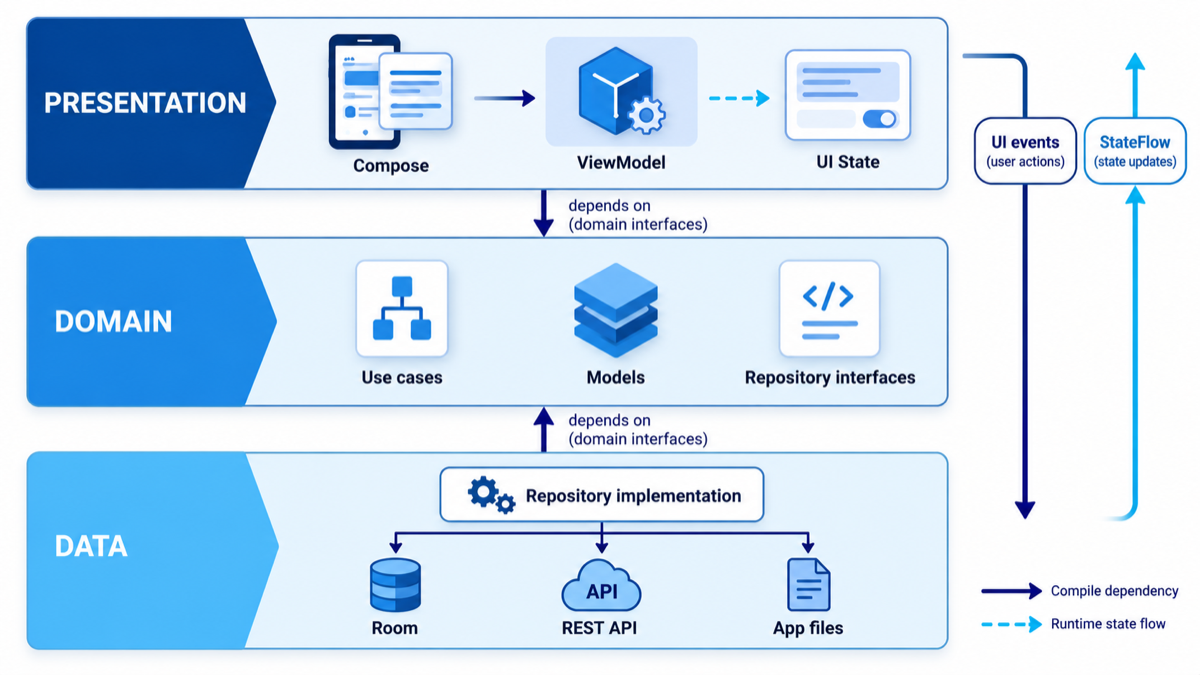
\includegraphics[width=\linewidth]{figures/Kiến trúc ba lớp.png}
\end{column}
\end{columns}
\end{frame}

% ------------------------------------------------------------
\subsection{Cấu trúc mô-đun}
% ------------------------------------------------------------
\begin{frame}{Cấu trúc mô-đun}
\begin{columns}[T]
\begin{column}{0.52\textwidth}
\footnotesize
\begin{itemize}\setlength{\itemsep}{3pt}
\item \textbf{:app} lắp ghép: MainActivity, shell, root routing, Hilt wiring
\item \textbf{Feature} sở hữu màn hình: mỗi phân hệ một module feature (video, music, news, games, onboarding, account\ldots)
\item \textbf{Domain, data và core} được quản lý riêng: domain một module Kotlin thuần; data theo phân hệ; core theo vai trò (design system, session, media, database, datastore, network)
\item Kiểm tra phụ thuộc \textbf{tự động} bằng tác vụ \texttt{verifyArchitecture}
\end{itemize}
\end{column}
\begin{column}{0.42\textwidth}
\centering
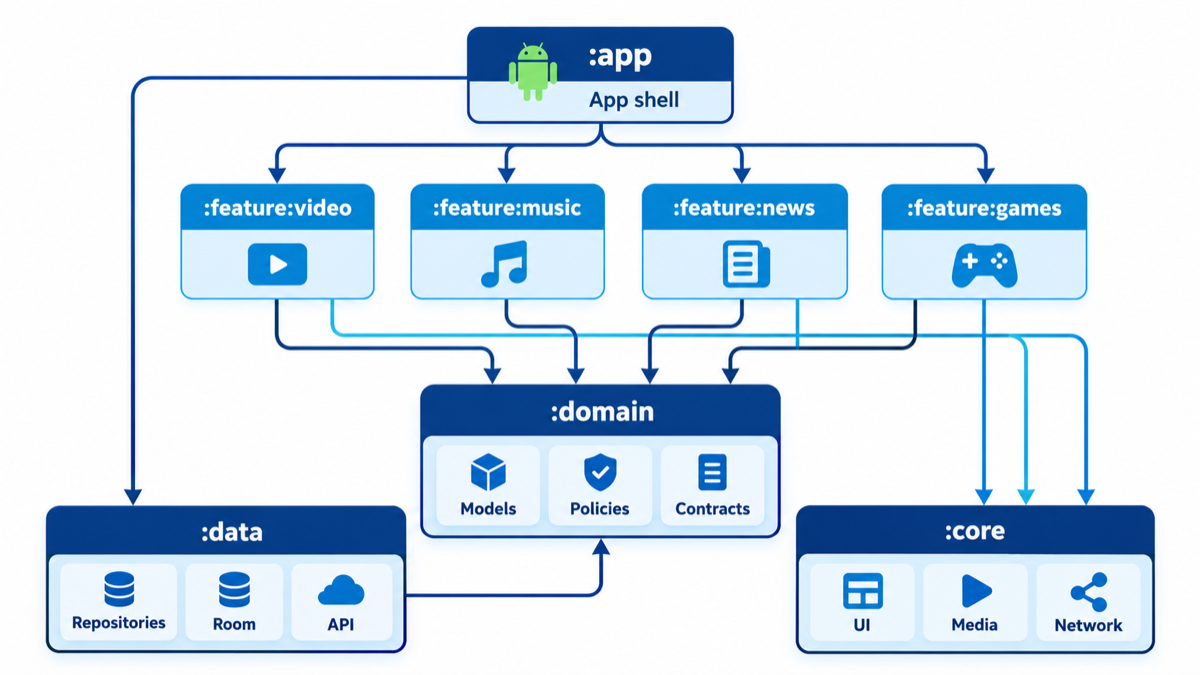
\includegraphics[width=\linewidth]{figures/Cấu trúc mô-đun.png}
\end{column}
\end{columns}
\end{frame}

% ------------------------------------------------------------
\subsection{Điều hướng do app quản lý}
% ------------------------------------------------------------
\begin{frame}{Điều hướng do app quản lý}
\centering
{\small App chọn luồng khởi động và quản lý Back. Feature cung cấp route và graph của mình.}\vspace{2.5mm}

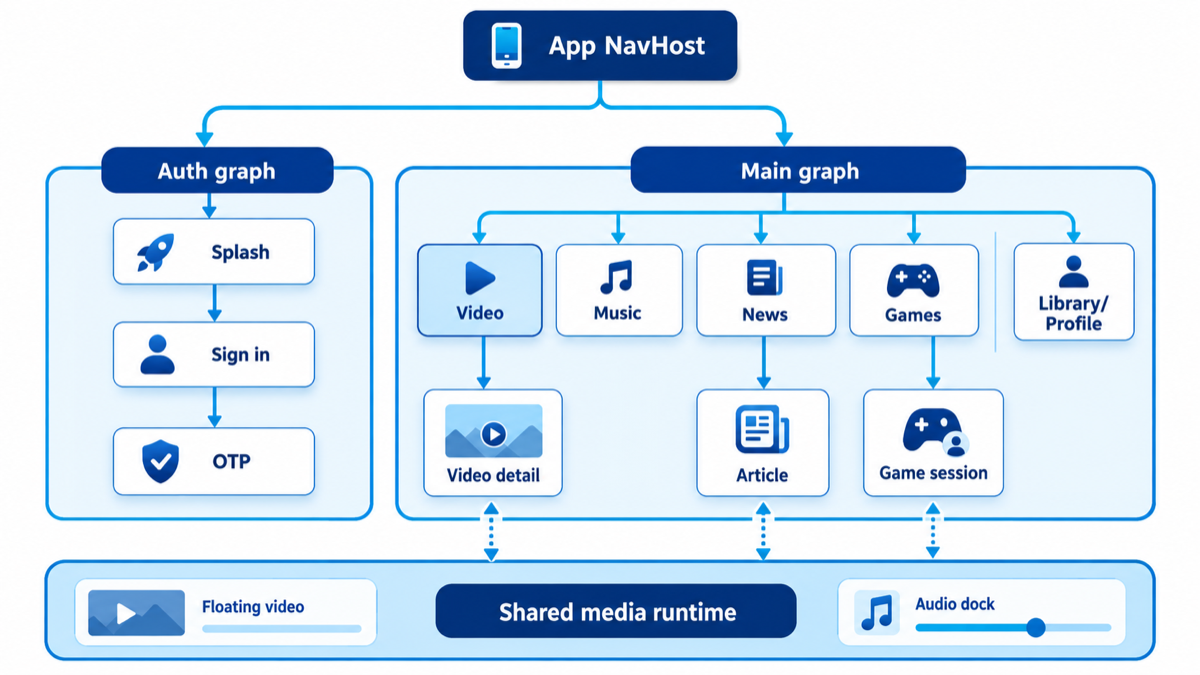
\includegraphics[width=10.5cm]{figures/Điều hướng do app quản lý.png}
\end{frame}

% ------------------------------------------------------------
\subsection{Nội dung và dữ liệu lấy từ đâu?}
% ------------------------------------------------------------
\begin{frame}{Nội dung và dữ liệu lấy từ đâu?}
\small
\centering
\begin{tabular}{@{}p{3.3cm}p{5.3cm}p{5.6cm}@{}}
\toprule
\textbf{Loại dữ liệu} & \textbf{Nguồn dự kiến} & \textbf{Ứng dụng nhận được gì?} \\
\midrule
Video và nhạc & Tệp nhóm tự tạo hoặc được phép dùng & Nhóm upload kho media, API trả danh mục \\
Bài đọc và nghe tin TTS & Bài nhóm biên soạn hoặc được phép lưu toàn văn & Nội dung để đọc trong app và tạo tiếng nói \\
Tin từ nguồn ngoài & Dự kiến RSS VnExpress, có ghi nguồn & Tiêu đề, tóm tắt và link về bài gốc \\
Game và dữ liệu tài khoản & Luật game trong app, cấu hình và API của nhóm & Quiz, nhiệm vụ, playlist và dữ liệu cá nhân \\
\bottomrule
\end{tabular}

\vspace{0.3cm}
{\footnotesize\color{TextGray} Kho nội dung mẫu trong phạm vi môn học: 50 video, 50 bài hát, 50 bài báo~--~tự dựng hoặc được phép dùng.}
\end{frame}

% ------------------------------------------------------------
\subsection{Upload và phát nội dung}
% ------------------------------------------------------------
\begin{frame}{Upload và phát nội dung}
\begin{center}
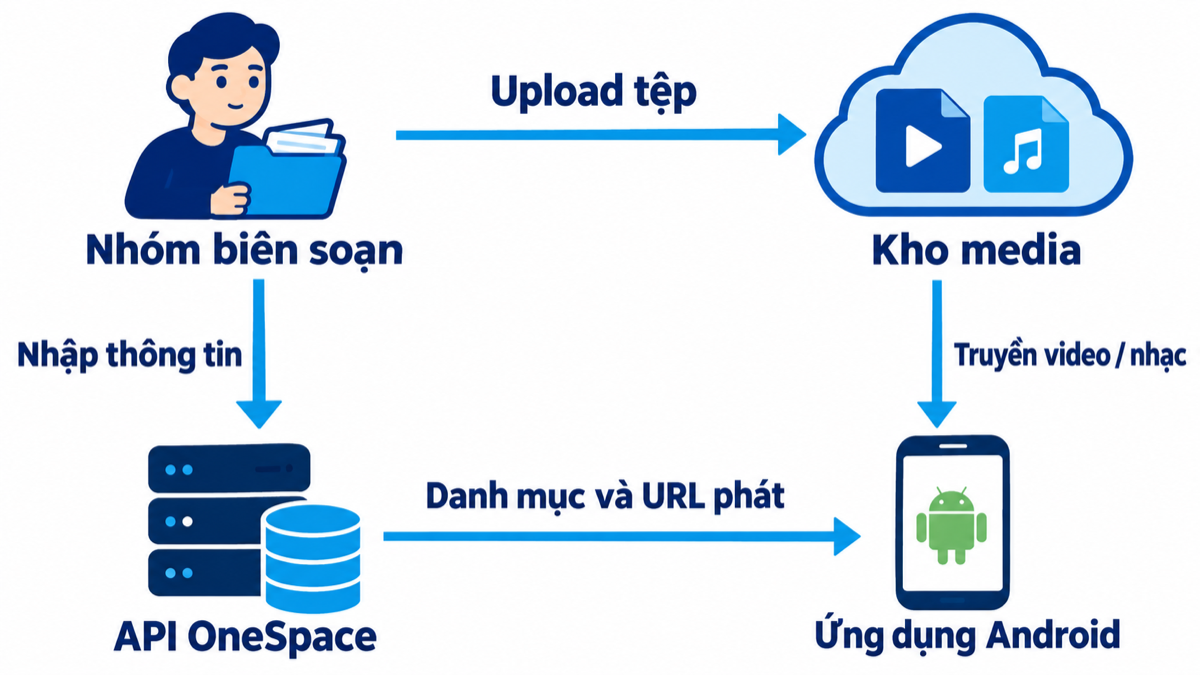
\includegraphics[width=8.2cm]{figures/Upload và phát nội dung.png}
\end{center}
\vspace{1.5mm}
\small
\begin{itemize}\setlength{\itemsep}{3pt}
\item App gọi API lấy danh mục (tiêu đề, mô tả, URL); media stream thẳng từ kho media qua bộ phát Media3
\item Thay nguồn $=$ thay URL: player, UI và logic phát không đổi
\item Quiz, nhiệm vụ, câu hỏi soạn sẵn đi kèm nội dung khi đăng
\end{itemize}
\end{frame}

% ------------------------------------------------------------
\subsection{Dữ liệu được lưu ở đâu?}
% ------------------------------------------------------------
\begin{frame}{Dữ liệu được lưu ở đâu?}
\small
\centering
\begin{tabular}{@{}p{3.0cm}p{5.4cm}p{5.6cm}@{}}
\toprule
\textbf{Nơi lưu} & \textbf{Dữ liệu chính} & \textbf{Ý nghĩa} \\
\midrule
Room trên điện thoại & Danh mục đã lấy, bookmark, tiến độ & Đọc lại dữ liệu đã lưu khi mất mạng \\
DataStore & Thiết lập nhỏ của thiết bị & Ghi nhớ cấu hình giao diện và phát \\
Tệp riêng của ứng dụng & TTS và MP3 đã tạo hoặc tải hoàn tất & Lưu tệp âm thanh, tách khỏi cache tạm \\
Server và kho media & Tài khoản, playlist đồng bộ, điểm và tệp gốc & Quản lý dữ liệu chung và quyền truy cập \\
\bottomrule
\end{tabular}

\vspace{0.3cm}
{\footnotesize\color{TextGray} Nguyên tắc offline-first: mọi dữ liệu đã xem có bản lưu cục bộ; đồng bộ lại khi có mạng.}
\end{frame}

% ------------------------------------------------------------
\subsection{Mô hình dữ liệu và API}
% ------------------------------------------------------------
\begin{frame}{Mô hình dữ liệu (physical) --- ERD Room schema v5}
\begin{center}
\begin{tikzpicture}[font=\tiny]
  % ===== video_progress =====
  \draw[draw=BKTemplate, thick] (0,0) rectangle (4.0,-1.45);
  \fill[BKTemplate] (0,0) rectangle (4.0,-0.3);
  \node[text=white, font=\tiny\bfseries] at (2.0,-0.15) {video\_progress};
  \node[anchor=north west, align=left, inner sep=3pt] at (0.03,-0.33) {\underline{videoId}~PK (FK logic)\\title\\positionMs (vị trí xem)\\updatedAt};
  % ===== watchlist =====
  \draw[draw=BKTemplate, thick] (4.3,0) rectangle (8.3,-1.3);
  \fill[BKTemplate] (4.3,0) rectangle (8.3,-0.3);
  \node[text=white, font=\tiny\bfseries] at (6.3,-0.15) {watchlist};
  \node[anchor=north west, align=left, inner sep=3pt] at (4.33,-0.33) {\underline{videoId}~PK (FK logic)\\title\\savedAt};
  % ===== point_entries (nhóm: gamification) =====
  \draw[draw=GreenOK!65!black, thick] (8.6,0) rectangle (12.6,-1.45);
  \fill[GreenOK!65!black] (8.6,0) rectangle (12.6,-0.3);
  \node[text=white, font=\tiny\bfseries] at (10.6,-0.15) {point\_entries};
  \node[anchor=north west, align=left, inner sep=3pt] at (8.63,-0.33) {\underline{id}~PK (tự tăng)\\source\\amount\\timestamp};
  % ===== daily_missions (nhóm: gamification) =====
  \draw[draw=GreenOK!65!black, thick] (0,-1.65) rectangle (4.0,-3.6);
  \fill[GreenOK!65!black] (0,-1.65) rectangle (4.0,-1.95);
  \node[text=white, font=\tiny\bfseries] at (2.0,-1.8) {daily\_missions};
  \node[anchor=north west, align=left, inner sep=3pt] at (0.03,-1.98) {\underline{id}~PK\\title\\targetType $\cdot$ target\\progress $\cdot$ completed\\date (mỗi ngày)};
  % ===== extracted_audio (nhóm: thư viện âm thanh) =====
  \draw[draw=BKLight, thick] (4.3,-1.65) rectangle (8.3,-3.35);
  \fill[BKLight] (4.3,-1.65) rectangle (8.3,-1.95);
  \node[text=white, font=\tiny\bfseries] at (6.3,-1.8) {extracted\_audio};
  \node[anchor=north west, align=left, inner sep=3pt] at (4.33,-1.98) {\underline{videoId}~PK (FK logic)\\title $\cdot$ creator\\url $\cdot$ duration\\extractedAt};
  % ===== downloaded_content (nhóm: thư viện offline) =====
  \draw[draw=BKLight, thick] (8.6,-1.65) rectangle (12.6,-3.35);
  \fill[BKLight] (8.6,-1.65) rectangle (12.6,-1.95);
  \node[text=white, font=\tiny\bfseries] at (10.6,-1.8) {downloaded\_content};
  \node[anchor=north west, align=left, inner sep=3pt] at (8.63,-1.98) {\underline{contentId}~PK (FK logic)\\type (video / nhạc / tin)\\title $\cdot$ subtitle\\downloadedAt};
  % ===== DataStore + tệp =====
  \node[draw=BKLight, thick, rounded corners=3pt, fill=BKLight!10, align=left, inner sep=4pt, anchor=north west, text width=11.2cm, font=\tiny] at (0.35,-3.95) {\textbf{DataStore (preferences):} phiên đăng nhập $\cdot$ cài đặt $\cdot$ bài tin đã lưu $\cdot$ playlist (JSON) $\cdot$ trạng thái game (streak, pet, shop)\\[1pt]\textbf{Tệp riêng của ứng dụng:} MP3 trích từ video, TTS đã tạo};
  \node[font=\tiny, text=TextGray, align=center, text width=12.4cm] at (6.3,-5.15) {videoId / contentId là khóa ngoại \textbf{logic} (tham chiếu mềm) tới danh mục; không có FK vật lý --- ràng buộc do repository trong app đảm bảo.\\ Màu tiêu đề: xanh đậm = tương tác nội dung $\cdot$ xanh lam = thư viện offline (tải về / trích xuất) $\cdot$ xanh lá = gamification.};
\end{tikzpicture}
\end{center}
\end{frame}

% ------------------------------------------------------------
\begin{frame}{Mô hình dữ liệu backend (thiết kế giai đoạn remote)}
\begin{center}\tiny
\setlength{\tabcolsep}{3pt}
\begin{tabular}{@{}p{2.4cm}p{2.6cm}p{4.4cm}p{3.5cm}@{}}
\toprule
\textbf{Entity} & \textbf{Khóa chính} & \textbf{Trường chính} & \textbf{Quan hệ} \\
\midrule
users & id & phone, name, avatar, created\_at & 1--n playlists, point\_entries, missions, progress \\
content\_items & id & type (video / nhạc / tin), title, url, duration, published\_at & 1--n playlist\_items, progress \\
playlists & id & user\_id, name, updated\_at & thuộc users; 1--n playlist\_items \\
playlist\_items & (playlist\_id, item\_id) & position & thuộc playlists; trỏ content\_items \\
point\_entries & id & user\_id, source, amount, created\_at & thuộc users (ledger điểm) \\
daily\_missions & id & user\_id, title, target, progress, date & thuộc users \\
progress & (user\_id, item\_id) & position\_ms, updated\_at & thuộc users + content\_items \\
\bottomrule
\end{tabular}
\end{center}
\vspace{1.2mm}
{\tiny\color{TextGray} Thiết kế cho giai đoạn remote (ADR-17)~--~chưa hiện thực; khớp endpoint ở slide sau. Bản đang chạy trên máy là ERD Room ở slide trước (6 bảng cục bộ).}
\end{frame}

% ------------------------------------------------------------
\begin{frame}{Thiết kế API (giai đoạn remote)}
{\tiny\color{TextGray} REST + JSON, HTTPS TLS 1.2 trở lên, token định danh (SEC-03). Thiết kế cho giai đoạn remote~--~app hiện dùng mock repository cùng interface nên thay thế không đụng UI.}
\vspace{1.2mm}
\begin{center}\tiny
\begin{tabular}{@{}llp{4.4cm}p{5.0cm}@{}}
\toprule
\textbf{Method} & \textbf{Endpoint} & \textbf{Ý nghĩa} & \textbf{Trả về chính} \\
\midrule
GET & /catalog/videos & Danh mục video & id, title, creator, duration, url, thumbnail \\
GET & /catalog/tracks & Danh mục nhạc & id, title, artist, album, duration, url \\
\midrule
GET & /news/articles & Danh sách tin & id, title, summary, source, publishedAt \\
GET & /news/articles/\{id\} & Chi tiết bài & toàn văn, quiz, bài liên quan \\
\midrule
POST & /auth/otp & Gửi OTP SMS & thời hạn 5 phút (SEC-01) \\
POST & /auth/verify & Đổi OTP lấy token & token, hồ sơ người dùng \\
\midrule
GET & /me/playlists & Playlist của tôi & id, tên, danh sách mục \\
POST & /me/playlists & Tạo / sửa playlist & playlist đã lưu \\
POST & /me/points & Ghi điểm, nhiệm vụ & số dư, nhiệm vụ hôm nay \\
\bottomrule
\end{tabular}
\end{center}
\vspace{0.5mm}
{\tiny\color{TextGray} Phân trang: \texttt{?page=\&limit=}; đồng bộ xung đột theo ID + version.}
\end{frame}

% ------------------------------------------------------------
\begin{frame}{API: mẫu phản hồi và xử lý mã lỗi}
\begin{columns}[T]
\begin{column}{0.42\textwidth}
{\small\textbf{Mẫu phản hồi}}\\[0.8mm]
{\tiny\ttfamily
GET /catalog/videos?page=1\\[0.5mm]
\{"items": [\\
~~"id": "v01",\\
~~"title": "Giới thiệu OneSpace",\\
~~"creator": "Nhóm OneSpace",\\
~~"duration": 213,\\
~~"url": "https://\ldots/oceans.mp4",\\
~~"thumbnail": "https://\ldots/v01.jpg"\\
], "page": 1, "hasMore": true\}}
\end{column}
\begin{column}{0.56\textwidth}
{\small\textbf{Mã lỗi chuẩn HTTP}}\\[0.8mm]
{\tiny
\begin{tabular}{@{}llp{4.4cm}@{}}
\toprule
\textbf{Mã} & \textbf{Ý nghĩa} & \textbf{App xử lý} \\
\midrule
400 & Sai tham số & Thông báo, giữ dữ liệu cũ \\
401 & Token hết hạn & Yêu cầu đăng nhập lại \\
403 & Không có quyền & Ẩn hành động cần quyền \\
404 & Không có nội dung & EmptyState + gợi ý thay thế \\
409 & Xung đột phiên bản & Giữ bản mới hơn, sync lại \\
429 & Quá nhiều request & Chờ rồi tự thử lại \\
5xx & Lỗi server & ``Không tải được'' + Thử lại \\
\bottomrule
\end{tabular}}
\vspace{1.5mm}

{\tiny\color{TextGray} Lỗi player và lỗi request hiện qua ErrorState dùng chung; connectivity chỉ là tín hiệu gợi ý~--~kết quả thao tác do lỗi thật quyết định.}
\end{column}
\end{columns}
\end{frame}

% ------------------------------------------------------------
\subsection{Luồng chính: sequence diagram}
% ------------------------------------------------------------
\begin{frame}{Sequence diagram: xung đột âm thanh (C1)}
\begin{center}
\begin{tikzpicture}[
  font=\tiny,
  ll/.style={draw=BKTemplate, thick, rounded corners=2pt, fill=BKTemplate!10, minimum width=2.15cm, minimum height=0.5cm, align=center},
  msg/.style={-{Latex[length=1.5mm]}, thick},
  ret/.style={-{Latex[length=1.5mm]}, thick, dashed},
  note/.style={draw=OrangeWarn, fill=OrangeWarn!12, rounded corners=2pt, inner sep=2.5pt, align=center}]
  \node[ll] (u)  at (1.1,6.45) {\bfseries Người dùng};
  \node[ll] (ui) at (3.9,6.45) {Màn Nhạc (UI)};
  \node[ll] (sp) at (6.8,6.45) {Session\\Coordinator};
  \node[ll] (mc) at (9.7,6.45) {Media\\Coordinator};
  \node[ll] (pl) at (12.55,6.45) {2 Player\\(nhạc $\cdot$ video)};
  \foreach \n in {u,ui,sp,mc,pl} \draw[dashed, TextGray!60] (\n.south) -- ++(0,-4.6);
  % Thanh kích hoạt (execution specification)
  \foreach \bx/\ya/\yb in {3.9/5.4/5.9, 6.8/1.75/5.4, 9.7/2.45/3.5, 12.55/2.45/3.0}{
    \draw[fill=white, draw=black!60, thick] (\bx-0.07,\ya) rectangle (\bx+0.07,\yb);}
  \draw[msg] (1.1,5.9) -- (3.9,5.9) node[midway, above]{1. Mở bài nhạc (video đang phát)};
  \draw[msg] (3.9,5.4) -- (6.8,5.4) node[midway, above]{2. Xin quyết định luồng tiếng};
  \node[note] at (8.6,5.0) {chưa có quy tắc đã lưu};
  \draw[dashed, TextGray] (6.8,5.28) -- (7.6,5.03);
  \draw[ret] (6.8,4.5) -- (1.1,4.5) node[midway, above]{3. Popup 2 lựa chọn + ô tick (F-COM-14)};
  \draw[msg] (1.1,4.0) -- (6.8,4.0) node[midway, above]{4. Chọn ``Tắt tiếng video''};
  \draw[msg] (6.8,3.5) -- (9.7,3.5) node[midway, above]{5. Áp dụng chính sách};
  \draw[msg] (9.7,3.0) -- (12.55,3.0) node[midway, above, align=center]{6. Video: còn hình,\\tắt tiếng};
  \draw[msg] (9.7,2.45) -- (12.55,2.45) node[midway, above, align=center]{7. Nhạc: phát tiếp,\\nguồn tiếng chính};
  \node[note] at (9.35,1.8) {tick ``Không hỏi lại'' $\Rightarrow$ lần sau áp dụng im lặng};
  \draw[dashed, TextGray] (6.8,2.1) -- (7.4,1.86);
\end{tikzpicture}
\end{center}
\vfill
{\tiny\color{TextGray} Lựa chọn còn lại: ``Dừng video''~--~video dừng và lưu vào Xem sau đúng vị trí.}
\end{frame}

% ------------------------------------------------------------
\begin{frame}{Sequence diagram: khởi động và khôi phục phiên}
\begin{center}
\begin{tikzpicture}[
  font=\tiny,
  ll/.style={draw=BKTemplate, thick, rounded corners=2pt, fill=BKTemplate!10, minimum width=2.15cm, minimum height=0.5cm, align=center},
  msg/.style={-{Latex[length=1.5mm]}, thick},
  ret/.style={-{Latex[length=1.5mm]}, thick, dashed},
  note/.style={draw=OrangeWarn, fill=OrangeWarn!12, rounded corners=2pt, inner sep=2.5pt, align=center}]
  \node[ll] (u)    at (1.1,6.45) {\bfseries Người dùng};
  \node[ll] (os)   at (3.9,6.45) {Hệ điều hành};
  \node[ll] (app)  at (6.8,6.45) {App\\(Splash $\rightarrow$ Main)};
  \node[ll] (st)   at (9.7,6.45) {DataStore\\+ Room};
  \node[ll] (ss)   at (12.55,6.45) {Session\\Coordinator};
  \foreach \n in {u,os,app,st,ss} \draw[dashed, TextGray!60] (\n.south) -- ++(0,-4.6);
  % Thanh kích hoạt
  \foreach \bx/\ya/\yb in {6.8/3.9/5.4, 9.7/4.4/4.9, 12.55/3.1/3.9}{
    \draw[fill=white, draw=black!60, thick] (\bx-0.07,\ya) rectangle (\bx+0.07,\yb);}
  \draw[msg] (1.1,5.9) -- (3.9,5.9) node[midway, above]{1. Mở lại app (sau khi tiến trình bị hủy)};
  \draw[msg] (3.9,5.4) -- (6.8,5.4) node[midway, above]{2. Khởi động process + MainActivity (splash giữ theo state)};
  \draw[msg] (6.8,4.9) -- (9.7,4.9) node[midway, above]{3. Đọc onespace\_session, hydrate playlist};
  \draw[ret] (9.7,4.4) -- (6.8,4.4) node[midway, above]{4. tab cuối, bài cuối, playlists, điểm/streak};
  \draw[msg] (6.8,3.9) -- (12.55,3.9) node[midway, above]{5. restoreColdStartSession(): mở tab cuối; đặt bài cuối ở 0:00};
  \node[note] at (10.85,3.02) {nhạc không tự phát\\--~bấm play trên dock};
  \draw[dashed, TextGray] (12.55,3.35) -- (12.1,3.08);
  \node[note, align=center] at (7.3,1.95) {Mở lại video dở: checkpoint Room 3 giây $\rightarrow$ seek đúng vị trí};
  \draw[dashed, TextGray] (9.7,2.2) -- (9.55,2.02);
\end{tikzpicture}
\end{center}
\vfill
{\tiny\color{TextGray} Đã đối chiếu code: tab cuối + bài cuối (trạng thái dừng) + playlist + vị trí video khi mở lại video + điểm/streak/pet giữ nguyên. Vị trí đọc tin và ván game qua process death, tự phát lại nhạc: hạng mục sau~--~xem bảng kiểm chứng kiến trúc trong báo cáo.}
\end{frame}

% ------------------------------------------------------------
\subsection{Phối hợp video, nhạc và các màn hình}
% ------------------------------------------------------------
\begin{frame}{Phối hợp video, nhạc và các màn hình}
\small
\begin{enumerate}\setlength{\itemsep}{5pt}
\item \textbf{Dùng chung bộ phát}~--~Một bộ phát video và một bộ phát audio phục vụ toàn ứng dụng (Media3); bốn phân hệ không tự dựng player riêng
\item \textbf{Chọn âm thanh chính}~--~Video có tiếng và nhạc cùng phát: hỏi người dùng giữ nguồn nào (popup C1/C2 kèm ô tick ``Không hỏi lại''); một thời điểm chỉ một nguồn tiếng chính
\item \textbf{Hiệu ứng game lớp riêng (F-GAME-13)}~--~SFX qua SoundPool sonification, tự giảm còn 25\% khi nhạc/video/TTS đang phát, mức âm chỉnh trong Cài đặt; không xin audio focus
\item \textbf{Giữ phiên khi chuyển màn hình}~--~Video nổi và audio dock tiếp tục điều khiển cùng phiên phát; quay lại đúng vị trí (lệch $\leq$ 2 giây), kể cả khi hệ điều hành đã hủy app
\end{enumerate}
\vspace{1mm}
\begin{exampleblock}{Kết quả}
Người dùng nghe nhạc khi đọc tin, xem video nổi khi lướt feed, chơi game với nhạc nền~--~một trải nghiệm liền mạch thay vì bốn ứng dụng riêng.
\end{exampleblock}
\end{frame}

% ------------------------------------------------------------
\begin{frame}{Sequence diagram: xem video và chuyển phân hệ (X1)}
\begin{center}
\begin{tikzpicture}[
  font=\tiny,
  ll/.style={draw=BKTemplate, thick, rounded corners=2pt, fill=BKTemplate!10, minimum width=2.15cm, minimum height=0.5cm, align=center},
  msg/.style={-{Latex[length=1.5mm]}, thick},
  ret/.style={-{Latex[length=1.5mm]}, thick, dashed},
  note/.style={draw=OrangeWarn, fill=OrangeWarn!12, rounded corners=2pt, inner sep=2.5pt, align=center}]
  \node[ll] (u)  at (1.1,6.45) {\bfseries Người dùng};
  \node[ll] (ui) at (3.9,6.45) {Màn Video (UI)};
  \node[ll] (sc) at (6.8,6.45) {Session\\Coordinator};
  \node[ll] (pv) at (9.7,6.45) {Video engine\\(Media3)};
  \node[ll] (sh) at (12.55,6.45) {Shell\\(cửa sổ nổi)};
  \foreach \n in {u,ui,sc,pv,sh} \draw[dashed, TextGray!60] (\n.south) -- ++(0,-4.6);
  % Thanh kích hoạt
  \foreach \bx/\ya/\yb in {3.9/4.35/5.9, 6.8/4.85/5.4, 9.7/4.35/4.95, 12.55/2.5/3.95}{
    \draw[fill=white, draw=black!60, thick] (\bx-0.07,\ya) rectangle (\bx+0.07,\yb);}
  \draw[msg] (1.1,5.9) -- (3.9,5.9) node[midway, above]{1. Chạm video trong feed};
  \draw[msg] (3.9,5.4) -- (6.8,5.4) node[midway, above, align=center]{2. playVideo(id): đọc vị trí đã lưu; nhạc đang phát $\rightarrow$ popup C2 (X0)};
  \draw[msg] (6.8,4.9) -- (9.7,4.9) node[midway, above]{3. Mở stream tại resumeFrom};
  \draw[ret] (9.7,4.4) -- (3.9,4.4) node[midway, above]{4. Phát tiếp tại vị trí đã lưu ($\leq$ 2 giây)};
  \draw[msg] (1.1,3.9) -- (12.55,3.9) node[midway, above]{5. Chọn tab khác (ví dụ Tin tức)};
  \node[note] at (10.8,3.05) {videoDocked = true\\cửa sổ nổi hiện, vẫn phát};
  \draw[dashed, TextGray] (12.55,3.5) -- (12.1,3.1);
  \draw[msg] (12.55,2.5) -- (3.9,2.5) node[midway, above]{6. Chạm ``Mở rộng'': mở lại player, cùng engine, đúng vị trí};
  \node[note] at (9.2,1.75) {Đóng cửa sổ nổi: dừng + lưu vị trí + thêm Xem sau};
  \draw[dashed, TextGray] (12.55,2.2) -- (10.85,1.8);
\end{tikzpicture}
\end{center}
\vfill
{\tiny\color{TextGray} Kịch bản theo code thật: OneSpaceApp (videoDocked), SessionPlayers (FloatingVideo), MediaPlaybackCoordinator (cùng engine). Tab đích là Home: phát trong card feed, không cửa sổ nổi.}
\end{frame}

% ------------------------------------------------------------
\subsection{Nghe tin TTS và tạo MP3}
% ------------------------------------------------------------
\begin{frame}{Nghe tin TTS và tạo MP3}
\begin{columns}[T]
\begin{column}{0.54\textwidth}
\footnotesize
\begin{itemize}\setlength{\itemsep}{3pt}
\item \textbf{TTS đọc bài báo:} nút ``Nghe tin'' trong trình đọc $\rightarrow$ TTS on-device đọc bài; nhạc đang phát tự nhường (C13)
\item \textbf{Tạo file MP3 thật:} bản audio của bài (TTS) và bản trích từ video (F-VID-10) được ghi thành tệp mp3 trong tệp riêng của ứng dụng
\item Tệp phát lại như một bài nhạc thường: điều khiển bằng dock mini, đưa vào hàng đợi, xoá được
\item Engine TTS là \textbf{module thay được}: on-device (miễn phí, chất lượng vừa) hoặc API cloud (chất lượng, phí theo ký tự)~--~đổi hướng không đụng UI
\end{itemize}
\end{column}
\begin{column}{0.40\textwidth}
\centering
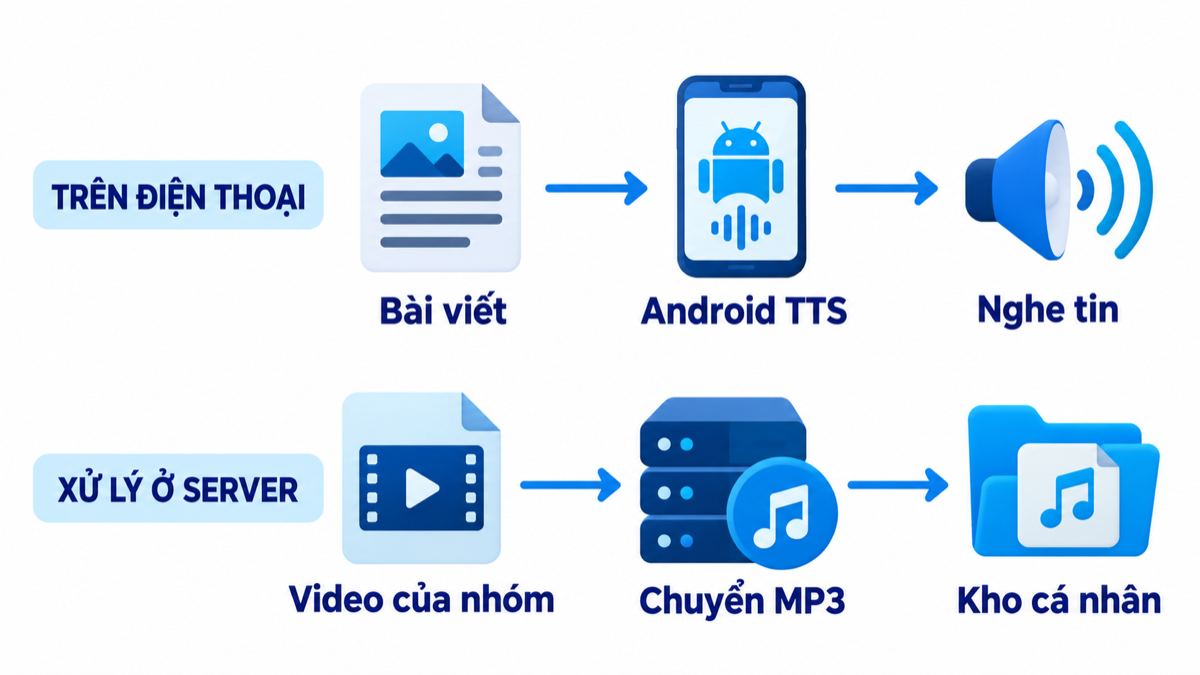
\includegraphics[width=\linewidth]{figures/Nghe tin TTS và tạo MP3.png}
\end{column}
\end{columns}
\end{frame}

% ------------------------------------------------------------
\subsection{Ma trận truy vết}
% ------------------------------------------------------------
\begin{frame}{Ma trận truy vết (requirement $\rightarrow$ kiến trúc)}
\begin{center}\tiny
\setlength{\tabcolsep}{3pt}
\begin{tabular}{@{}p{4.0cm}p{3.0cm}p{2.5cm}p{3.8cm}@{}}
\toprule
\textbf{Yêu cầu (kèm user story)} & \textbf{Use case} & \textbf{Màn hình} & \textbf{Thành phần kiến trúc} \\
\midrule
F-VID-01 · US-VID-01 & Xem video (UC-02) & Mockup F-VID-01 & feature/video + core/media \\
F-VID-08 · US-VID-02, US-CROSS-03 & Tiếp tục xem khi chuyển phân hệ (X1) & Mockup F-VID-08 & app (shell) + core/session \\
F-MUS-02 · US-MUS-02, US-CROSS-01 & Nghe nhạc (UC-03) & Mockup F-MUS-02 & core/session + core/media \\
F-COM-14 · US-MUS-03, US-CROSS-02 & Xử lý xung đột âm thanh (X0) & Mockup F-COM-14 & domain (SessionPolicy) + app \\
F-NEWS-05 · US-NEWS-04, US-CROSS-08 & Nghe tin TTS (X4) & Mockup F-NEWS-05 & feature/news + core/media (TTS) \\
F-GAME-02 · US-GAME-02 & Chơi minigame (UC-05) & Mockup F-GAME-02 & feature/games + core/media \\
F-COM-01 · US-COM-01 & Quản lý danh tính (UC-11) & Mockup F-COM-01 & feature/auth + core/datastore \\
\bottomrule
\end{tabular}
\end{center}
\vspace{1.5mm}
{\tiny\color{TextGray} Chuỗi đầy đủ: yêu cầu $\rightarrow$ use case (sơ đồ tổng quan) $\rightarrow$ user story kèm AC $\rightarrow$ màn hình (mock up ảnh thật) $\rightarrow$ module kiến trúc. Tổng: \textbf{76} yêu cầu $\rightarrow$ \textbf{45} story (100\% có AC) $\rightarrow$ \textbf{74} mã có ảnh chụp $\rightarrow$ \textbf{23} mô-đun Gradle.}
\end{frame}
